% =============================================================================
% REMOVED FROM body.tex BY THE 2026-09-11 COMPACTION PASS. NOT \input BY EITHER
% BUILD. DO NOT COMPILE. This file exists so the companion paper on the residual
% audit can be assembled without git archaeology.
%
% Provenance: every block below is copied verbatim out of docs/paper/body.tex as
% it stood at commit d0ba530 ("Withdraw the mechanism claim, and correct two
% numbers that came from a bug"), with the original line ranges recorded above
% each block. The theorem section it belongs with,
% docs/paper/sections/residual_floor_theorem.tex, was left untouched in the
% repository and is likewise no longer \input.
%
% What the manuscript kept: a single subsection (sec:residual) reporting the
% floor at the truth (mean 0.192 on 200/200 cases, uniform freestream exactly
% zero), the 200/200 descent-from-truth result, the 24/24 iterate-selection
% result, and the acceptance-gate measurement. Everything below is the detail
% that was removed from it.
%
% Labels used below that no longer exist in body.tex, and must be re-declared or
% re-pointed when this material is reassembled:
%   sec:floor_ladder  sec:descent  sec:regime  tab:floor_ladder  tab:descent200
%   tab:iters  fig:fig4  tab:positioning  sec:residual_floor  thm:residual-floor
%   thm:consistency-floor  prop:kernel  sec:rf_operator
% =============================================================================


% -----------------------------------------------------------------------------
% BLOCK 1 -- Related Work, "Learned solver-correctors and the 'fixer' premise".
% Original body.tex lines 228-268. The compacted manuscript keeps a three-sentence
% version of this paragraph; the operator-consistency argument and the floor-share
% measurement below were removed with it.
% -----------------------------------------------------------------------------

\paragraph{Learned solver-correctors and the ``fixer'' premise.} Several lines of work
use the discretised residual or a coarse-solution error as a \emph{correction
objective}: learned PDE solvers with convergence guarantees \citep{hsieh2019neuralpde},
deep-equilibrium operators for steady PDEs \citep{marwah2023fnodeq}, iterative refiners
\citep{lippe2023pderefiner}, learned residual-error correctors
\citep{learned2023residualcorrection}, and---most recently---training-free correction
that solves a linearised inverse problem on the PDE residual at each rollout step,
reporting up to $100\times$ error reduction on transient benchmarks
\citep{huang2025physicscorrect}. PINNs \citep{raissi2019pinn} embed the residual
in the training loss. NeuroForge implements a contractive DEQ corrector and a
feed-forward residual-conditioned corrector squarely in this family. \textbf{Our
contribution to this line is to test the residual-as-correction premise head-on and find it
does not hold.} As a correction \emph{objective}---where a step must reduce the
residual---residual minimisation does not track error minimisation on a real RANS benchmark:
descending $J=\tfrac12\|R_h\|^2$ from the exact ground truth cuts the residual to $39.8\%$
of its starting value while driving the field error up on $200/200$ cases, and on
$94$--$98\%$ of cases started from the deployed backbone. And when the residual is fed as
an input \emph{feature} to a corrector supervised toward ground truth, a controlled
ablation attributes the gain to the learned correction rather than to the residual input
(\autoref{sec:v2}). The residual's value is as a
\emph{trust signal}---it ranks which predictions to distrust---not as a correction
mechanism telling you \emph{how} to fix them; the learned correction does the fixing.
The prior successes and our negative are consistent, and what separates them is the
\emph{operator}, not the problem class. Residual-driven correction works where the
monitored residual is the solver's own, hence (near-)exact at the true solution:
resolved transient PDEs stepped on their training grid \citep{huang2025physicscorrect},
variational problems with certified residuals \citep{learned2023residualcorrection},
and---on steady CFD, so the boundary is demonstrably not steady versus
transient---a Newton--Krylov correction driven by the solver's own residual, which
lowers it by seven orders of magnitude \emph{while} reducing field and aerodynamic
error \citep{lei2026newtonkrylov}. It fails where the monitor is instead a
surrogate-side operator that a deployed system can afford, inconsistent with the one
that produced the labels. Carrying \emph{some} floor is not sufficient for that
failure---every discrete monitor carries one---so the operative quantity is how much
of a prediction's score the floor already accounts for. On the deployed arm the median
truth-to-prediction residual ratio is $0.864$: \textbf{$86\%$ of a typical
prediction's score is present at zero error}, a fraction set by the operator rather
than the model, which prices the certificate rather than invalidating it
(\autoref{sec:conformal}). The floor is a necessary condition for the failure mode
we report, and the prior successes operate where it is absent. Our negative is scoped
to that deployment-realistic regime.


% -----------------------------------------------------------------------------
% BLOCK 2 -- Related Work, "Residual-based, data-free error signals".
% Original body.tex lines 270-305. The compacted manuscript keeps the first three
% sentences and the three-part contribution list; the a-posteriori-estimation
% argument below was removed.
% -----------------------------------------------------------------------------

\paragraph{Residual-based, data-free error signals.} Closest to our \emph{trust-signal}
half is recent work that reads the PDE residual as a reference-free indicator of prediction
error. \citet{roy2025anchor} use a physics-informed, residual-based error estimator to detect
and correct accumulating error in neural-operator \emph{time-marching}, triggering a classical
solver when the estimator fires; \citet{song2026structureaware} design an epistemic-UQ scheme
whose uncertainty bands are aligned with localised residual structure in operator surrogates.
\citet{gopakumar2025pre} go furthest in the trust direction: they use the PDE residual itself
as a conformal nonconformity score, obtaining data-free coverage guarantees---in
\emph{residual} space, with the transfer to solution space left open as a set-propagation
problem. Our residual-floor theorem (\autoref{sec:residual_floor}) supplies a concrete
mechanism for that gap in the discrete steady-RANS setting: the monitored residual has a
nonzero floor at the reference solution and a kernel of undetectable modes, so residual-space
smallness cannot by itself certify solution-space accuracy. The question we put to the residual---can a quantity computable without the true
solution certify that solution's accuracy?---is the defining question of
a-posteriori error estimation, and the classical answer is instructive: residual
magnitude is not itself an error estimate, and becomes one only when weighted by the
solution of an adjoint problem measuring how strongly each local residual propagates
into the functional of interest \citep{beckerrannacher2001dwr}. The neural analogue
keeps that structure: \citet{hillebrecht2025posteriori} bound the true error of a
PDE-defined PINN by its residual scaled by a stability constant of the underlying
operator. Both results are conditional on a property our monitor does not have---that
the residual vanishes at the exact solution---and the residual-floor theorem is
precisely a statement of how that condition fails for an under-resolved discrete
steady-RANS operator. That is why we use the residual to \emph{rank} cases rather than
to \emph{bound} them, and obtain the bound from conformal calibration instead.
From the theory side,
\citet{mukherjee2026certification} prove that vanishing residuals guarantee solution
convergence only under additional compactness assumptions; our setting is the practical
complement, where the discrete monitored residual provably does \emph{not} vanish at the
dataset truth. We share the premise that the residual is a data-free error signal and do not
claim to originate it. Our distinct contributions are (i)~the head-to-head \emph{dissociation}---the residual is a
good trust signal but a poor correction objective, established on the same steady-state RANS
benchmark; (ii)~the \emph{residual-floor theorem} establishing a nonzero continuum limit for
the floor and characterising the undetectable kernel modes; and (iii)~a split-conformal certificate calibrated on
the \emph{deployed, corrected} field. Our setting is steady-state external aerodynamics with
per-case spatial trust, rather than time-marching error control.


% -----------------------------------------------------------------------------
% BLOCK 3 -- the positioning table and the paragraph that introduced it.
% Original body.tex lines 380-440 (Section 2.1, "Positioning").
% -----------------------------------------------------------------------------

\autoref{tab:positioning} places the neighbouring work on the boundary that secondary
result draws. The organising question there is not which features a system has, but
whether the residual it drives is the \emph{same discrete operator} that produced its
reference data. Where it is, residual-driven correction works and is already
demonstrated. Where an affordable surrogate-side proxy stands in for it, the truth itself
fails the check.

\begin{table}[t]
\centering
\small
\caption{The boundary, and where the closest 2024--2026 work sits on it. The
discriminating question is whether the residual being monitored or minimised is the
discrete operator whose root the reference solution is. Where it is, the floor at the
truth is zero by construction and minimising the residual is minimising the error. Where
it is not---the affordable, deployment-time case, where a cheap proxy operator stands in
for the generator's---the floor is nonzero and the objective's minimiser is displaced from
the truth, which we test by explicitly minimising $J=\tfrac12\|R_h\|^2$ at $n=200$ under
three step rules, not by observing a supervised corrector. Prior residual-correction
successes and this paper's negative result are not in
conflict; they sit on opposite sides of this line.}
\label{tab:positioning}
\begin{adjustbox}{max width=\textwidth}
\begin{tabular}{p{0.17\textwidth} p{0.36\textwidth} p{0.40\textwidth}}
\toprule
 & \textbf{Solver-consistent operator} & \textbf{Surrogate-side proxy operator} \\
\midrule
Floor at the truth
 & Zero by construction.
 & Nonzero, with a nonzero continuum limit (\autoref{sec:residual_floor}); it
   \emph{grows} under refinement, $p=-0.387$, rising in $21/24$ cases
   (\autoref{sec:floor_ladder}). \\
\addlinespace
Residual as a correction objective
 & Works: residual $\downarrow$ and error $\downarrow$ together \citep{lei2026newtonkrylov, huang2025physicscorrect, learned2023residualcorrection}.
 & Fails: descent from the exact truth drives the field error up on $200/200$ cases
   under Armijo-line-searched gradient descent, and on $94$--$98\%$ of cases started
   from the deployed backbone ($p<10^{-30}$, unchanged under three step rules); the
   residual-selected iterate is never the error-optimal one, in $24/24$ cases
   (\autoref{sec:descent}). \\
\addlinespace
Residual as an error detector
 & Not the question these works ask.
 & Positive across backbones, but matched by a physics-free score on field error;
   it wins outright only on drag (\autoref{sec:selective}). \\
\addlinespace
Cost at deployment
 & A solver-grade operator per correction step.
 & ${\sim}1.1$\,ms per case (\autoref{sec:cost}), which is why it is the one a
   deployed surrogate can actually afford. \\
\bottomrule
\end{tabular}
\end{adjustbox}
\end{table}

The trust-layer components this paper retains---distribution-free conformal bands
\citep{gopakumar2025pre, jia2026multigranularity}, residual-based error signals
\citep{roy2025anchor, song2026structureaware} and a-posteriori certification
\citep{mukherjee2026certification}---are individually well developed in that recent
literature, and we claim no priority over them. What is new here is the measurement that
constrains all of them: the operator such a layer can afford to monitor does not vanish on
the data it is calibrated against, and that gap is not a resolution artifact.


% -----------------------------------------------------------------------------
% BLOCK 4 -- the iteration sweep. Original body.tex lines 1551-1615 (subsection
% sec:iters, "The iteration sweep: cutting the error buys no residual reduction"),
% plus its figure caption from lines 2288-2298. The compacted manuscript keeps
% only the acceptance-gate measurement that followed this material.
% -----------------------------------------------------------------------------

\subsection{The iteration sweep: cutting the error buys no residual reduction}
\label{sec:iters}

The direct evidence that the residual is a poor \emph{objective} is the descent experiment
of \autoref{sec:descent}, which minimises it. This subsection reports a weaker,
complementary observation---an iteration sweep on a single trained checkpoint
(\autoref{tab:iters})---and the four limits that keep it from carrying the claim alone.

\paragraph{Four limits of this sweep.} \emph{(i)} The swept
knob is the DEQ corrector's internal fixed-point cap
(\texttt{results/sensitivity/iters.json}), and that corrector is trained by supervised
regression toward ground truth; it never sees the residual as an objective. The sweep is
therefore an anti-correlation along one trajectory, not a test of residual minimisation.
\emph{(ii)} The anti-correlation is carried by one channel. Across the sweep the residual rises while surface
$\texttt{mse\_p}$ falls, and those two are strongly anti-correlated (rank correlation
$-0.94$); $\texttt{mse\_u}$ has essentially no relationship with the residual
($-0.03$). $\texttt{mse\_u}$ falls only over iterations $0\!\to\!3$ and then
\emph{rises} alongside the residual ($2.287\to2.575$ against $0.542\to0.620$), so on
three of the five intervals the two move in the \emph{same} direction. Row $0$ is
moreover backbone-only, which makes $0\!\to\!1$ a corrector on/off contrast rather than
an iteration step; restricted to $n_{\mathrm{iters}}\ge1$ the residual rises $84.7\%$
while $\texttt{mse\_u}$ rises $4.7\%$---again the same direction. The
$0\!\to\!3$ $\texttt{mse\_u}$ endpoints alone therefore
overstate the effect. \emph{(iii)} It is a single unseeded checkpoint ($n=1$), and it reports
$\texttt{mse\_u}$ and surface $\texttt{mse\_p}$ only, while \autoref{tab:indist} shows
this corrector family inflating $\texttt{mse\_v}$ and volume $\texttt{mse\_p}$.
\emph{(iv)} A seeded five-seed re-run on the Transolver$+$DEQ arm
(\texttt{scripts/iters\_sweep\_seeded.py}, $24$ cases) returns \textsc{direction-only}
against a bar declared in advance: the residual is higher at $k{=}15$ in $5/5$ seeds but
by only $+1.5\%$, at $1.3\times$ the across-seed standard deviation where we required
$2\times$; it is monotone in $0/5$ seeds; and paired per case it is higher in only
$45/120=38\%$. The sweep therefore supports \emph{decoupling}, not divergence, and we
claim only that cutting field error along this path buys no residual reduction. None of
these limits applies to \autoref{sec:descent}, which is why the claim now rests there.

\begin{table}[t]
\centering
\small
\caption{Iteration sensitivity sweep: \texttt{results/sensitivity/iters.csv}. Single
sweep (one checkpoint, not seeded). See \autoref{fig:fig4}.}
\label{tab:iters}
\begin{tabular}{r r r r r}
\toprule
\texttt{n\_iters} & $\texttt{mse\_u}$ & surf.\ $\texttt{mse\_p}$ & residual\_norm & resid$\leftrightarrow$err $\rho$ \\
\midrule
0  & $3.924$ & $541204$ & $0.113$ & $0.423$ \\
1  & $2.460$ & $428560$ & $0.336$ & $0.644$ \\
3  & $2.287$ & $336718$ & $0.542$ & $0.647$ \\
5  & $2.439$ & $308381$ & $0.594$ & $0.675$ \\
10 & $2.570$ & $300298$ & $0.618$ & $0.703$ \\
15 & $2.575$ & $300664$ & $0.620$ & $0.710$ \\
\bottomrule
\end{tabular}
\end{table}

As the loop iterates, the \textbf{PDE residual norm rises monotonically}
($0.11\rightarrow0.62$) while the \textbf{field error falls} ($\texttt{mse\_u}$
$3.92\rightarrow2.29$ by iter 3)---over that initial interval the two objectives move in
\emph{opposite} directions. Beyond iteration $3$ they move together, as noted above, so
the reading this table supports is that the residual is not a usable stopping signal
along this path rather than that it is anti-correlated with error throughout. (Note this
does not contradict the
DEQ contraction of \autoref{sec:conformal}: the contraction is in the correction variable
$\delta$, which converges; the PDE residual of the \emph{output field} is a different
quantity, and it is the one that rises.)

\begin{figure}[t]
\centering
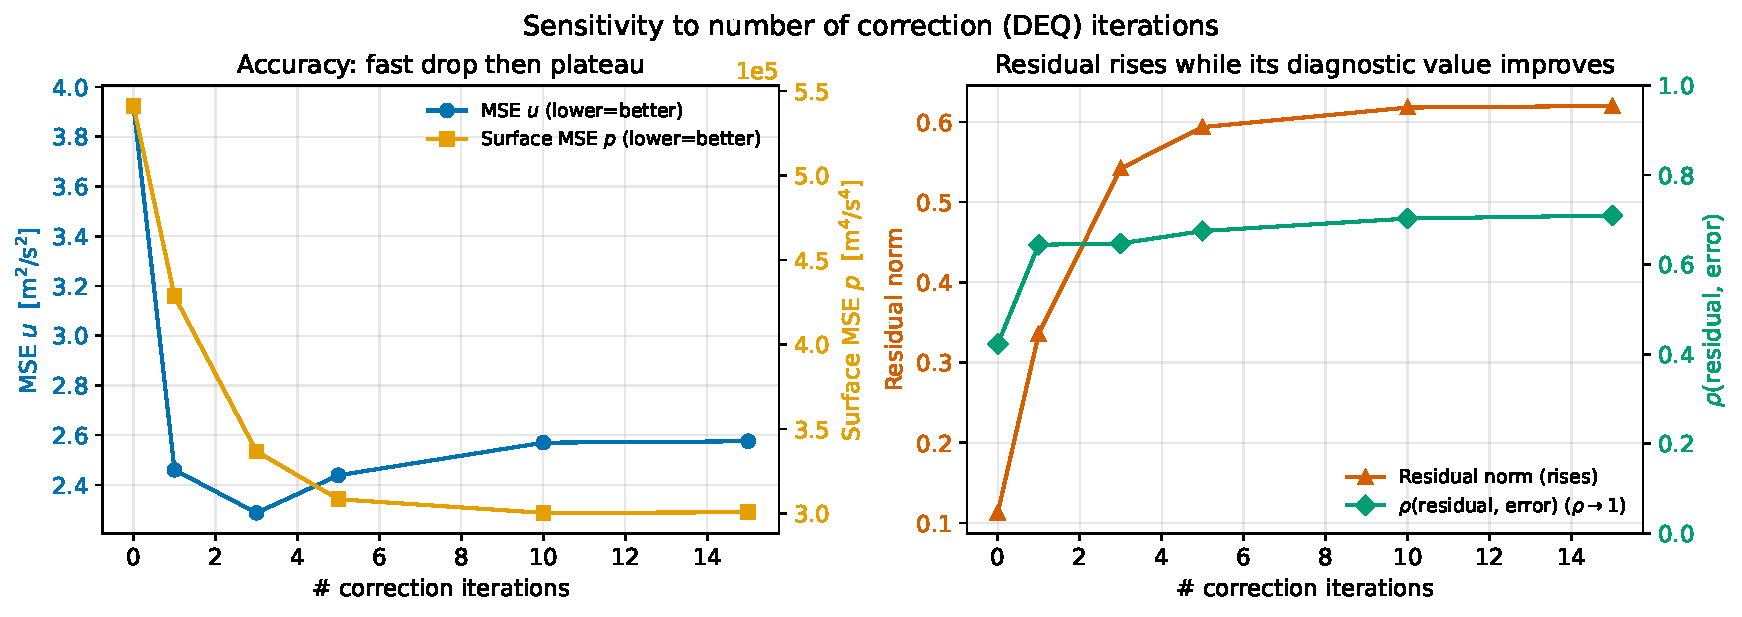
\includegraphics[width=0.85\textwidth]{../../results/figures/fig4_sensitivity_iters.pdf}
\caption{The iteration sweep (\autoref{tab:iters}, one
unseeded checkpoint). Over iterations $0\!\to\!3$ the PDE residual rises while
$\texttt{mse\_u}$ falls; beyond iteration $3$ the two move together. A seeded five-seed
re-run returns \textsc{direction-only}, so this figure illustrates \emph{decoupling}
between the residual and the error, not divergence. The claim itself rests on
\autoref{sec:descent}.}
\label{fig:fig4}
\end{figure}

% The following paragraph sat immediately after the acceptance-gate controls in
% body.tex (original lines 1650-1660) and was removed with the sweep it refers to.

This does not rescue the
residual as an \emph{objective}---the full step still raises the residual on half the
deployed cases while error falls, and \autoref{tab:iters} shows the two decoupled
under iteration. The gate and the objective are different mechanisms and earn separate
verdicts. (Scope: a single gated step applied counterfactually to
the deployed DEQ correction, which the shipped DEQ path bypasses by design; not a re-run of
the multi-iteration feed-forward loop of \autoref{tab:indist}, whose corrector checkpoints
were not retained.) We
additionally note that for the DEQ corrector the trust-gating and acceptance-test toggles
are structural no-ops---the DEQ branch bypasses both---so the only live correction knob is
the applied-delta step size (\texttt{results/sensitivity/toggles.json}).


% -----------------------------------------------------------------------------
% BLOCK 5 -- "The floor does not refine away". Original body.tex lines 1674-1760,
% including tab:floor_ladder.
% -----------------------------------------------------------------------------

\subsubsection{The floor does not refine away}
\label{sec:floor_ladder}

If the floor $r^\star=R_h(u^\star)$ were an artifact of the $128^2$ grid
under-resolving the boundary layer, everything built on it would collapse to ``you
under-resolved your data''. It is not. We rasterise the same AirfRANS truth at
$128^2$, $256^2$ and $512^2$ and measure the floor on each
(\texttt{scripts/floor\_resolution\_ladder.py}). Three choices were registered before
the run: the scored region is fixed in \textbf{physical} units (fluid cells with
$\mathrm{sdf}\ge 1.5\,h_{128}=0.0352$ chord), so refinement cannot manufacture a plateau
by unmasking the steepest cells; the reading of the fitted exponent in
$\|r^\star\|\sim Ch^{p}$ was fixed as $p\ge1$ is \textsc{decay} and $p<0.5$ is
\textsc{plateau}; and levels finer than the source cloud's own spacing are excluded. The
floor \emph{rises} as the grid is refined (\autoref{tab:floor_ladder}):
$0.0624\to0.0779\to0.1067$ while $h$ falls $4\times$, rising in $\mathbf{21/24}$ cases,
at $p=-0.387$---not merely inside the \textsc{plateau} band but the wrong \emph{sign}
for decay. A second, independent $16$-case five-rung implementation finds it decaying in
$0$ of $16$. (These band-restricted values are smaller than the whole-grid RMS floor of
mean $0.192$ quoted in \autoref{sec:residual_floor}; the two score different regions.)
Meanwhile $\|R_h(u_\infty)\|=0$ exactly at every level, because a spatially constant
field has identically zero finite differences at any $h$---so the gap by which the
objective prefers a wrong field to the truth widens as the grid improves.

\begin{table}[t]
\centering
\caption{The residual floor under grid refinement, $24$ AirfRANS test cases, scored on
a region fixed in physical units. The floor grows; the uniform freestream stays at
exactly zero. Fitted $p$ in $\|r^\star\|\sim Ch^{p}$; the pre-registered rule reads
$p<0.5$ as a plateau.}
\label{tab:floor_ladder}
\begin{tabular}{lccccc}
\toprule
level & $h$ & $\|r^\star\|$ & continuity & momentum & $\|R_h(u_\infty)\|$ \\
\midrule
$128^2$ & $0.0234$ & $0.0624$ & $0.0477$ & $0.0401$ & $0$ \\
$256^2$ & $0.0117$ & $0.0779$ & $0.0589$ & $0.0510$ & $0$ \\
$512^2$ & $0.0059$ & $\mathbf{0.1067}$ & $0.0791$ & $0.0717$ & $0$ \\
\midrule
fitted $p$ & & $-0.387$ & $-0.365$ & $-0.419$ & --- \\
rose in & & $21/24$ & $21/24$ & $21/24$ & --- \\
\bottomrule
\end{tabular}
\end{table}

\paragraph{Four controls, because a rising floor is usually a bug.}
\emph{The operator is second order.} Method of manufactured solutions on the same
monitor gives $p=2.06$ in the interior band ($2.02\pm0.05$ across per-case fits), so the
discretisation converges as claimed and the behaviour on real data is a statement about
the data. The manufactured field is a potential flow, on which the monitored viscous
term vanishes identically, so this control bounds truncation error and is \emph{not}
evidence that the operator is consistent (\autoref{sec:residual_floor}).
\emph{Restoring the omitted closure term does nothing.} Adding
$(\partial_j\nu_t)(\partial_j u_i+\partial_i u_j)$ back changes each rung's mean floor
by $-0.01\%$ to $+0.18\%$ across five rungs, and no individual case by more than
$1.5\%$; the term itself is $3.5$--$4.8\%$ of the floor. At $Re\approx2\times10^6$ the
entire viscous term is $1$--$4\%$ of convection, so no part of it can carry a floor of
this size.
\emph{A higher-order interpolant does not reduce it.} Rasterising the same source cloud
with cubic rather than linear interpolation \emph{raises} the floor by $6$--$12\%$, and
lowers it in only $2$--$4$ of $16$ cases. That control bears on the second-derivative
block---$5$--$7\%$ of the floor---and not on the first-derivative block carrying
$93$--$95\%$ of it, so we do not present it as the sharpest control.
\emph{The pipeline null, reported in full because its fine end reverses.} Pushing a
manufactured analytic solution through the identical rasteriser gives a residual that
falls over the ladder as a whole (fine/coarse $0.41$--$0.74$), but it reaches a minimum
at $256^2$ and then \emph{rises}, in $16/16$ cases, at $p=-0.49\pm0.14$ against the real
truth's $-0.58$ over the same rungs. At $512^2$ the pure-truncation curve is $10.9\%$ of
the raster curve in amplitude and $1.2\%$ in mean square, so over that range the raster
numbers are the pipeline-induced component to better than $1\%$. The null therefore does
\emph{not} show that the rasteriser cannot manufacture a rising residual; it shows that
on a field smooth at the cloud scale the effect is ${\sim}280\times$ smaller than on the
real data.

\paragraph{What this leaves.} Two statements, which we keep separate. The inconsistency
of the monitored operator gives the floor a nonzero \textbf{continuum limit}, so
refinement alone cannot remove it (\autoref{sec:residual_floor}). Its measured
\textbf{size} has two contributions we can name and cannot separate: the mismatch
between our Cartesian stencil and the body-fitted discrete balance the AirfRANS
reference actually solved, and the reconstruction of that reference onto our grid---at
fixed $h$, thinning the source point cloud eightfold raises the floor in $16/16$ cases,
on every band and at both rungs
(\texttt{results/certificates/floor\_cloud\_decimation.json}). The lockstep of
continuity and momentum does not discriminate between them, and no measurement we have
separates their shares. We therefore report both and attribute neither. A limitation of
the ladder itself: at $512^2$ the raster spacing is only $1.27\times$ the source cloud's
far-field spacing, so that level is near the exclusion limit; the $128^2\!\to\!256^2$
leg, comfortably clear of it, already shows the rise.


% -----------------------------------------------------------------------------
% BLOCK 6 -- "Descending the residual directly". Original body.tex lines 1762-1857,
% including tab:descent200. The compacted manuscript keeps the 24/24 and 200/200
% headline numbers and the rho-regime exception in two sentences; everything else
% below was removed.
% -----------------------------------------------------------------------------

\subsubsection{Descending the residual directly}
\label{sec:descent}

Testing the residual as an objective requires minimising it, which the corrector sweep of
\autoref{tab:iters} does not do: that corrector is trained by supervised regression toward
ground truth and never sees the residual as an objective. We minimise it directly, with
no network in the loop (\texttt{scripts/residual\_descent.py},
\texttt{scripts/residual\_descent\_test.py}).

\paragraph{The truth is not a fixed point.} Over $24$ AirfRANS cases, $300$ Adam steps
on $J(y)=\tfrac12\|R_h(y)\|^2$ started at the \textbf{exact ground truth}---so the
standard reply that a surrogate is over-smoothed has nothing to attach to---cut the
monitored residual by $84\%$ in $\mathbf{24/24}$ cases while driving the field error
from exactly zero to a median of $0.91$, the range in which a trained backbone
\emph{starts}. This is \autoref{thm:residual-floor}(ii) as a measurement: the same
descent applied to the \emph{error} objective from the same point does not move at all,
because $\nabla\|e\|^2=0$ there exactly while $\nabla J\ne0$. The compact-stencil
monitor falls in $24/24$ cases too, so this is not the differentiable twin's wider
Laplacian being gamed. Descent terminates at a residual of $0.028$ while the exact truth
sits at $0.110$: the objective ranks a field with error $1.31$ as four times better than
the field with error zero.

\paragraph{What holds universally is iterate selection.} We do \emph{not} claim residual
descent always harms the field: from a perturbed start it \emph{reduces} error in
$18/24$ cases, typically by $60\%$, before overshooting. What holds universally is a
statement about \textbf{iterate selection}. The error-minimising and residual-minimising
iterates never coincide---they differ in $24/24$ cases on both arms---and the
residual-selected iterate is strictly worse in $\mathbf{24/24}$. From the perturbed
start the error bottoms at step ${\approx}62$ while the residual keeps falling to step
${\approx}192$, by which point the error is $1.3\times$ its best value on the path. A
practitioner who stops where the residual says lands worse than a point already
traversed.

\paragraph{At $n=200$, on the deployed backbone, under gradient descent.} We repeated
the experiment with the framework's \emph{monitored} operator (a differentiable replica
verified against \texttt{Diagnostics.residual\_norm} to $10^{-8}$ relative), under
\textbf{Armijo-line-searched gradient descent}---so $J$ is monotone non-increasing and
the step is chosen by the objective---on $200$ cases, from the \emph{deployed}
Transolver (three seeds) and from the dropout-FNO of \autoref{tab:iters}, with the
far-field and near-wall Dirichlet data \emph{pinned at ground truth} so the negative
cannot be blamed on an unconstrained residual (\autoref{tab:descent200}). Unpinning
makes the negative stronger, not weaker ($100/99.5/100\%$ of cases across seeds), so the
pinned arm is the conservative one and is what we report. From the truth, $J$ falls to
$39.8\%$ of $J_0$ while field error rises on $\mathbf{200/200}$ cases and never returns
to its starting value at any of $500$ steps, ending at $1.57\times$ the \emph{entire}
error of the deployed Transolver. From the deployed Transolver the residual falls $34\%$
while the error rises on $\mathbf{96.5/94.0/98.0\%}$ of cases (median
$+76.5/+73.9/+86.9\%$; Wilcoxon $p<10^{-30}$), against the supervised corrector's
$-9/-21/-25\%$ on the same backbone. The verdict is unchanged under three step
rules---Armijo, fixed $\eta$ swept over $12$ decades, and Adam---and in each the outcome
is monotone in the \emph{achieved} $J$: the harder the objective is minimised, the worse
the field.

\begin{table}[t]
\centering
\small
\caption{Armijo-line-searched gradient descent on the monitored objective
$J=\tfrac12\|R_h\|^2$, $500$ steps, $n=200$ AirfRANS \texttt{full} test cases, with the
far-field and near-wall Dirichlet data pinned at ground truth. $J$ is monotone
non-increasing by construction. rel-$L_2$ is the fluid-masked rel-$L_2$ of speed (the
\texttt{measure\_acceptance\_gate} formula); $\Delta$ is the median per-case change.
$\|R_h\|$ here is the whole-grid norm, so the truth's $0.191$ is the same measurement as
the fluid-cell $0.192$ quoted elsewhere, rescaled by the geometric factor $0.995$.
\texttt{scripts/residual\_descent\_test.py}.}
\label{tab:descent200}
\begin{adjustbox}{max width=\textwidth}
\begin{tabular}{l r r r r r}
\toprule
start field & $\|R_h\|$ start$\to$end & $J/J_0$ & $\Delta$ rel-$L_2$ & frac.\ worse & $\texttt{mse\_u}$ start$\to$end \\
\midrule
ground truth $u^\star$ & $0.191\to0.125$ & $0.398$ & --- ($0\to0.0069$) & $\mathbf{200/200}$ & $0.000\to0.499$ \\
Transolver seed 0      & $0.218\to0.144$ & $0.406$ & $+76.5\%$ & $0.965$ & $0.119\to0.556$ \\
Transolver seed 1      & $0.218\to0.142$ & $0.388$ & $+73.9\%$ & $0.940$ & $0.120\to0.553$ \\
Transolver seed 2      & $0.217\to0.141$ & $0.390$ & $+86.9\%$ & $0.980$ & $0.103\to0.544$ \\
dropout-FNO            & $0.286\to0.153$ & $0.238$ & $-18.7\%$ & $0.250$ & $0.898\to0.930$ \\
\bottomrule
\end{tabular}
\end{adjustbox}
\end{table}

\paragraph{Where descent helps, and why that does not rescue the objective.} The
dropout-FNO row is a genuine exception: there descent \emph{lowers} the error, on $75\%$
of cases. The boundary is measurable in the theorem's own variable
$\rho=\|R_h(\hat u)\|/\|r^\star\|$. Over $200$ cases the fraction on which descent lowers
$\mathrm{rel}\text{-}L_2$ rises monotonically with $\rho$: for the dropout-FNO $0.40$ at
$\rho\in[1,1.5)$, $0.97$ at $[1.5,2)$ and $1.00$ above $2$; for the deployed Transolver
$0.01$, $0.28$, $0.25$. The deployed backbone has median $\rho=1.13$--$1.14$ with $88\%$
of cases in the lowest bin: it is already inside the regime where descent almost never
helps. ($\rho$ is a strong trend, not a complete predictor, so we claim the ordering and
not a law.) Even in the favourable regime the objective is unusable: the gain is
${\approx}1/35$ of the supervised corrector's, and there is \textbf{no stopping
rule}---$J$ falls monotonically on $100\%$ of cases while the error minimum is interior
on $78.5\%$. Two readings we record because they went against our expectation: the error
does not rise monotonically, so the claim is about endpoints and not paths; and the
iterate moves \emph{away} from the uniform freestream, so the damage does not require
reaching the spurious global minimum of leg~(i).


% -----------------------------------------------------------------------------
% BLOCK 7 -- "The boundary is the operator, not the problem class".
% Original body.tex lines 1859-1886. The compacted manuscript keeps the first
% clause of this argument in one sentence inside sec:residual.
% -----------------------------------------------------------------------------

\subsubsection{The boundary is the operator, not the problem class}
\label{sec:regime}

Residual-driven correction is not doomed in general, and it matters to say exactly where
it works. \citet{lei2026newtonkrylov} take a surrogate prediction as an initial guess
for Newton--Krylov correction on \emph{steady} CFD and lower the median residual $L_2$
ratio by over seven orders of magnitude \emph{while} substantially reducing field and
aerodynamic error---residual down and error down, on steady problems as here;
\citet{huang2025physicscorrect} report the same on transient rollouts. That is not a
counterexample to our result, it locates it. In those works the residual being driven is
the \emph{solver's own} discrete operator, the one whose root the reference solution is,
so its floor at the truth is zero by construction and minimising the residual is
minimising the error. Our monitor is the affordable surrogate-side one: a different
discretisation, on a different mesh, from the generator of the labels. Its floor is not
zero, does not vanish under refinement (\autoref{sec:floor_ladder}), and its minimiser is
displaced from $u^\star$ (\autoref{sec:residual_floor}). We therefore draw the boundary
at \textbf{operator consistency}; the obvious alternatives---steady versus transient,
resolved versus under-resolved---are falsified by \citet{lei2026newtonkrylov} being
steady and successful.

The observation that a PDE residual need not vanish at the ground truth is not ours
alone: \citet{zhang2026phymgn} report it for shock physics and conclude that a
physics-informed loss ``cannot be formulated using the absolute PDE residual alone;
instead, it must be defined relative to the residual present in the ground-truth
data''. Their remedy requires $R_h(u^\star)$, which a deployment-time monitor does not
have. Our contribution relative to theirs is to establish that the floor has a nonzero
continuum limit for an inconsistent operator, to measure that refinement does not remove
it, and to show what the resulting misplaced minimum does to a correction path.


% -----------------------------------------------------------------------------
% BLOCK 8 -- the floor's effect on certificate width. Original body.tex lines
% 1964-1986 (inside sec:conformal). The compacted manuscript keeps the coverage,
% the 6.5-7.9x width, the 11.33x floor-subtraction reversal and the 2.34x
% headroom number in three sentences; the surrounding argument was removed.
% -----------------------------------------------------------------------------

\paragraph{What the floor costs the certificate: valid, but wide.} The certificates above
are stated on field-error targets. The quantity an engineer actually wants bounded is a
force coefficient, and conformalising the monitored residual against $|\Delta C_D|$ shows
exactly what the floor does to a certificate that remains formally valid. Over $400$
random half-splits at a $0.90$ target on the deployed backbone
(\texttt{results/review/functional\_audit\_gate\_followup.json}), coverage comes out at
$0.901$--$0.903$ across three seeds---so the guarantee holds, and the floor does
\emph{not} invalidate split conformal, which needs only exchangeability and never
supposed the score vanished at the truth. What the floor destroys is tightness. The median
bound is $\mathbf{6.5}$--$\mathbf{7.9\times}$ the median drag error it certifies. We
tested the obvious explanation---that the floor is what makes it wide---and it is
\emph{wrong}. Removing the floor exactly, by scoring the field difference
$\|R_h(\hat u)-R_h(u^\star)\|$, makes the bound \textbf{wider} ($7.35\times$ to
$11.33\times$, $3/3$ seeds; a scale-invariance gate passes at exactly $0.0$, so this is
not an artifact of the counterfactual score having a smaller median). What sets the
width is the heavy tail of the drag error itself: its $0.9$ quantile is $15.1\times$ its
median, so a score carrying no information at all would give $15.1\times$. Against that
reference the monitor is worth $\mathbf{2.34\times}$, and that---not the floor---is the
honest statement of what it buys. \autoref{sec:floor_ladder} closes the obvious escape: the
floor does not decay under refinement, so a finer grid does not narrow this certificate.
This is the precise sense in which the audit can certify and yet not
certify usefully, and it is why we describe the residual's certification role as priced
rather than absent.
